\documentclass[a4paper]{article}

\usepackage{fontspec}
\usepackage{mathpazo}
\setmainfont
     [ BoldFont       = texgyrepagella-bold.otf ,
       ItalicFont     = texgyrepagella-italic.otf ,
       BoldItalicFont = texgyrepagella-bolditalic.otf ]
     {texgyrepagella-regular.otf}
\setmainfont{Gill Sans MT}

\usepackage[english]{babel}
\usepackage[utf8]{inputenc}
\usepackage{amsmath}
\usepackage{graphicx}
\usepackage[colorinlistoftodos]{todonotes}
\usepackage{physics}

%\DeclareMathOperator{\Tr}{Tr}

\title{Homework 3 : Aircraft Collision Avoidance Analyses using Reachability}

\author{David McPherson}

\date{\today}

\begin{document}
\maketitle

\section{Linear Velocity Control}
Consider a system of two airplanes (Dubin's vehicles) careening through the sky on a collision course.
Our two planes can only control their linear velocity and cannot escape into a veering mode.
This no-turning system defined in terms of relative coordinates is:

\begin{align*}
     \dot{x}_r    &= -u + d cos(\psi_r)
  \\ \dot{y}_r    &=  d sin(\psi_r)
  \\ \dot{\psi}_r &=  0
\end{align*}

We can use Ian Mitchell's "Toolbox of Level Set Methods" to perform reachability analysis on this system.
We will modify the default example Matlab script "air3D" that comes with his ToolboxLS.
We will need to change the functions defining the Hamiltonian ("air3DHamFunc") and the Hamiltonian's maximum partials ("air3DPartialFunc").

\subsection{MATLAB Function: HamFunc}

We need to find the optimal Hamiltonian so we can program it into the "air3DHamFunc" function.
Let us recast the bounds on the controls $u$ and $d$ as:

\begin{align*}
  \underline{v_1} &= c_u - o_u \\
  \bar{v_1}       &= c_u + o_u \\
  \underline{v_1} &= c_d - o_d \\
  \bar{v_1}       &= c_d + o_d \\
\end{align*}

So that $c_u$ is the center of the region $U$ and $o_u$ is the offset from the center to either end of the interval $U$.
Accordingly, $c_d$ is the center of $D$ and $o_d$ is the offset to either end of $D$.

Now, note that the system dynamics can be re-cast into a control-affine form:

\begin{align*}
  \dot{z}
  =
  \left[\begin{matrix} \dot{x}_r \\ \dot{y}_r \\ \dot{\psi}_r \end{matrix}\right]
  =
  \left[\begin{matrix} -u + d cos(\psi_r) \\ d sin(\psi_r) \\ 0 \end{matrix}\right]
  =
  \left[ \begin{matrix} 0 \\ 0 \\ 0 \end{matrix}\right] + \left[ \begin{matrix}-1 \\ 0 \\ 0\end{matrix}\right] u +\left[\begin{matrix} cos(\psi_r) \\ sin(\psi_r) \\ 0 \end{matrix}\right] d
\end{align*}

This allows us to decouple the effects of the input and output and optimize each individually.
   The corresponding (non-optimum) Hamiltonian is:

\begin{align*}
  \underset{u}{\max} \underset{d}{\min} H(z,p,u,d) =  p^T f(z,u,d) = -p_1 u + (p_1 cos(\psi_r) + p_2 sin(\psi_r)) d
\end{align*}

The optimum controls will always push the boundary of their set, depending on the sign of their coefficient.
For example, for $u$ to maximize the Hamiltonian it should assume it's minimum value when it's coefficient is negative ($-p_1 < 0)$, and $u$ should assume it's maximum value when it's coefficient $-p_1 > 0$.
The converse is true for $d$ as it seeks to minimize the Hamiltonian.
Thus we can obtain expressions for the ideal controls $u$ and $d$ as:

\begin{align*}
  u^* &= c_u + o_u sign(-p_1) \\
  d^* &= c_d + o_d sign(p_1 cos(\psi_r) + p_2 sin(\psi_r))
\end{align*}

Using these optimal controls in the Hamiltonian retursn the Optimal Hamiltonian as:

\begin{equation}
  H^*(z,p) = \underset{u}{\max} \underset{d}{\min} H(z,p,u,d) = H(z,p,u^*,d^*)
  = -c_u p_1 + o_u | p_1 |
  + (p_1 cos(\psi_r) + p_2 sin(\psi_r)) c_d - o_d |p_1 cos(\psi_r) + p_2 sin(\psi_r)|
\end{equation}

This is the Hamiltonian that was used in the $air3DHamFunc$ Matlab script.

\subsection{MATLAB Function: PartialHamFunc}
The second utility functions the Lax Friedrichs approximation requires for simulating the reachable set is a function which approximates:

$$
\alpha_i(z) = \underset{p}{\max} \left| \frac{\delta}{\delta p_i} H^*(z,p) \right|
$$

\subsection{Results}
With the requisite utility MATLAB functions defined corresponding to the particualars of our problem, our script is ready to roll.
The generated sets that reach the unsafe set are shown in the following figures for four different relative angles.

\begin{figure}[!ht]
  \centering
  \begin{minipage}[b]{0.4\textwidth}
    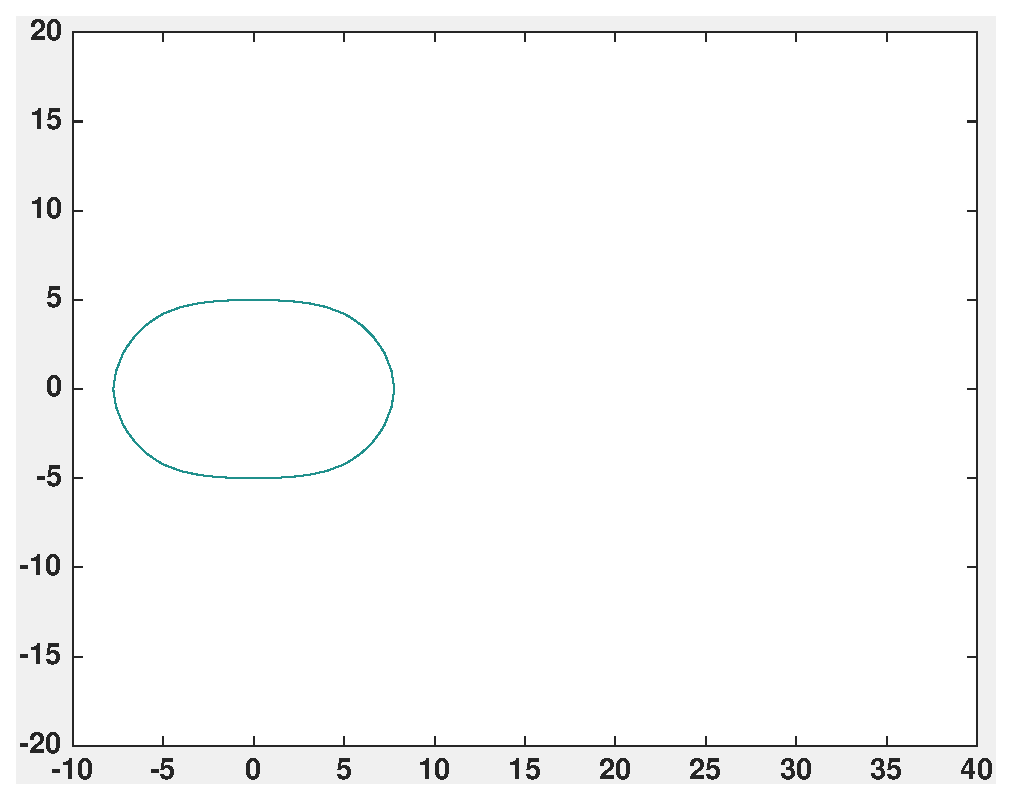
\includegraphics[width=1.0\textwidth]{velCont_psi1.eps}
    \caption{Unsafe set for Relative Angle $\psi_r = \frac{\pi}{2}$}
  \end{minipage}
  \hfill
  \begin{minipage}[b]{0.4\textwidth}
    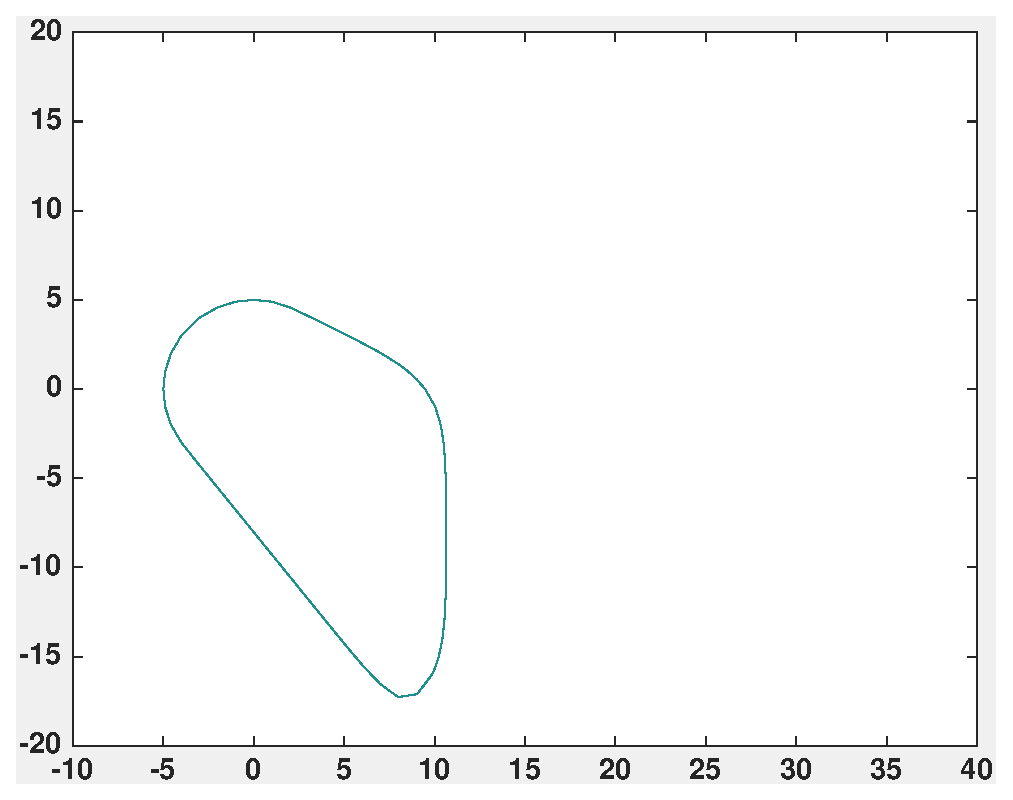
\includegraphics[width=1.0\textwidth]{velCont_psi13.eps}
    \caption{Unsafe set for Relative Angle $\psi_r = 0$}
  \end{minipage}
\end{figure}

\begin{figure}[!ht]
  \centering
  \begin{minipage}[b]{0.4\textwidth}
    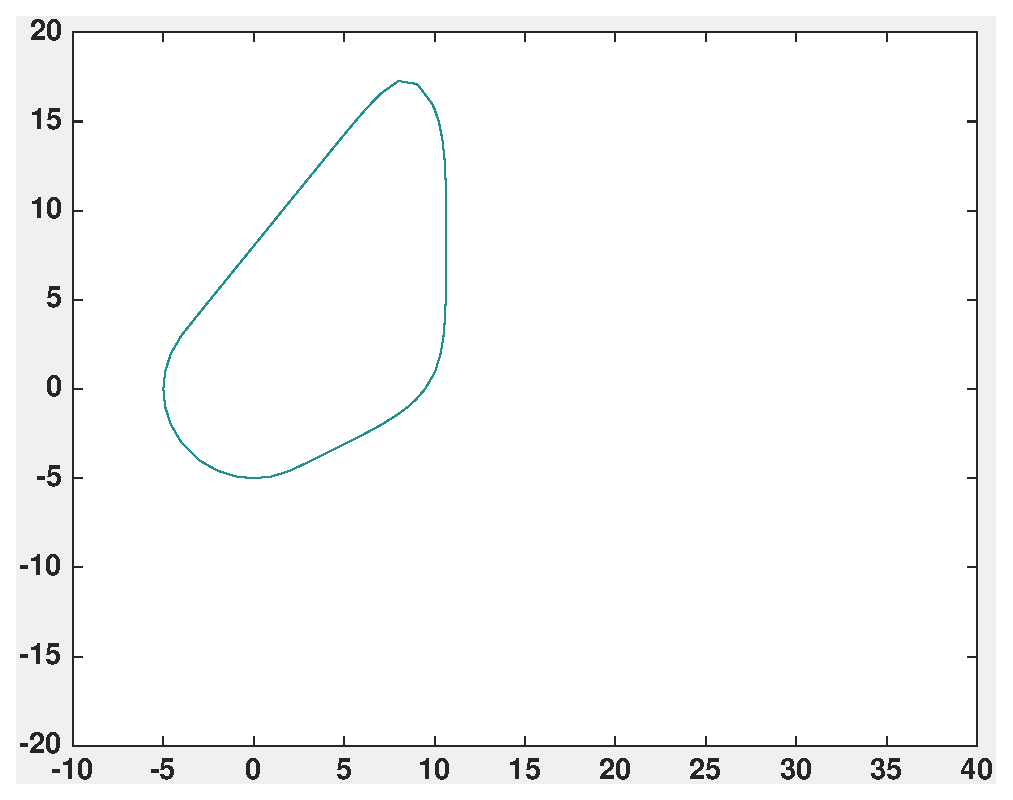
\includegraphics[width=1.0\textwidth]{velCont_psi37.eps}
    \caption{Unsafe set for Relative Angle $\psi_r = -\frac{\pi}{2}$}
  \end{minipage}
  \hfill
  \begin{minipage}[b]{0.4\textwidth}
    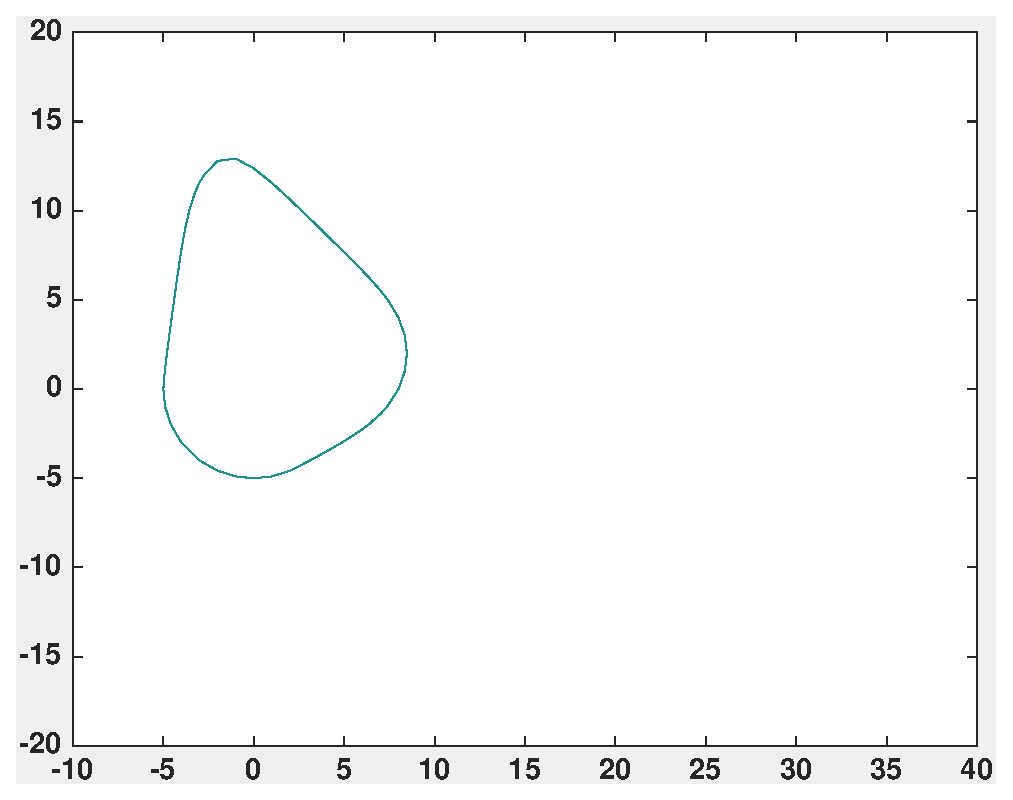
\includegraphics[width=1.0\textwidth]{velCont_psi43.eps}
    \caption{Unsafe set for Relative Angle $\psi_r = -\frac{\pi}{4}$}
  \end{minipage}
\end{figure}

As the time horizon $T \rightarrow \infty$ the reachable set reached a fixed point and ceased to expand.

\section{Mode Switching Control}

\end{document}
